\documentclass[a4paper,12pt]{article}
\usepackage[T1]{fontenc}
\usepackage[utf8]{inputenc}
\usepackage[italian]{babel}
\usepackage{hyperref}
\usepackage[]{graphicx}
\usepackage{hyperref}
\usepackage{fancyhdr}
\usepackage{lastpage}
\begin{document}


\title{Relazione progetto sito web Centro Commerciale Tito Levi Civita}
\begin{titlepage}
	\pagestyle{empty}
	\centering
	\vfill
	{
		\bfseries
		\vskip2cm
		\Large Università di Padova\\
		\Large Corso di laurea in informatica
		\vfill
		\Large Progetto per il corso di tecnologie web\\
		\Huge Centro Commerciale Torre Archimede\\
		\vfill
		
		\begin{figure}
			\centering
			
\includegraphics[width=0.6\linewidth]{images/LogoPadova}
		\end{figure}
		A cura di:\\
		\Large Giovanni Bergo:		1126144\\ Bianca Ciuche:		1122193 \\Daniel Rossi:		1125444\\ Manfredi Smaniotto:	1123057\\
		\vfill
		Sito web hostato all'indirizzo: \url{http://tecweb1617.studenti.math.unipd.it/darossi/mainPage/HTML/index.php}\\
		\vfill
	}
\end{titlepage}
\tableofcontents
\pagestyle{empty}
\newpage
\pagestyle{fancy}
\fancyhead[RE,LO]{}
\fancyfoot[CE,CO]{}
\fancyfoot[LE,RO]{Pagina \thepage\ di \pageref{LastPage}}
\section{Informazioni di accesso}
Il sito è accessibile al seguente link:
\begin{center}
	http://tecweb2016.studenti.math.unipd.it/darossi
\end{center}
Come primo account amministratore è possibile utilizzare:
\begin{itemize}
	\item username: admin
	\item password: admin
\end{itemize}
Vi sono anche alcuni account per utenti negozio come ad esempio:
\begin{itemize}
	\item username: lego
	\item password: lego
\end{itemize}
Dal pannello amministratore è possibile aggiungere account; non è concessa la connessione con due account contemporaneamente poichè le variabili di sessione vengono mantenute fino al logout successivo (non è stato possibile implementare un servizio automatico di refresh dell'orario di login all'interno della tabella account per poter verificare ad ogni cambio pagina l'effettiva attività dell'utente; nel database è comunque possibile trovare il codice di implementazione affinchè sia possibile l'inserimento di tale servizio una volta acquisiti i permessi di root).
\section{Scopo del progetto e target}
\subsection{Scopo del progetto}
Il progetto si pone l'obbiettivo di creare un sito internet di un centro commerciale, dove devono essere disponibili le principali informazioni riguardanti orari di apertura, offerte, prodotti dei negozi, comunicazioni di servizio e le indicazioni per raggiungere il centro commerciale. \\
L'utente web può quindi ricevere informazioni come sopra elencato utilizzando sia piattaforme desktop che dispositivi mobile.\\
Il proprietario del negozio ha invece la possibilità di accedere ad una sezione dedicata nell'area riservata dove poter personalizzare il proprio sito modificando gli orari di apertura, inserendo offerte, prodotti, le immagini e le descrizioni da presentare.\\
L'utente amministratore può invece gestire gestire tutti gli account presenti all'interno della piattaforma e scrivere alcune comunicazioni da dare ai clienti riguardo al centro commerciale.\\
\subsection{Target di utenza}
Il target del sito risulta essere l'utenza visitatrice dei centri commerciali, quindi un pubblico molto vasto ed eterogeneo che richiede la creazione di un sito adatto a tutti e senza particolari adattamenti per una particolare tipologia di pubblico.\\
Unica reale attenzione per la parte pubblica è stata l'organizzazione dei contenuti fondamentali sulla home, lasciando ad una navigazione più approfondita la ricerca di prodotti e promozioni.\\
La parte privata è invece pensata appositamente per un utilizzatore con buone conoscenze informatiche e indirizzato ad un utilizzo della piattaforme prettamente da computer fisico (fatichiamo a pensare che sia desiderato fare delle modifiche al sito da dispositivo mobile).
\section{Organizzazione delle informazioni}
\subsection{Introduzione}
I contenuti informativi presenti all'interno del sito sono stati organizzati in modo tale da lasciare le informazioni di maggiore importanza come le comunicazioni di servizio, gli orari e le ultime promozioni nella home del sito.\\
L'utente più curioso ha comunque modo di approfondire la propria navigazione ricercando offerte e promozioni nelle varie pagine raggiungibili tramite vari passaggi all'interno del sito (normalmente non vengono richiesti più di tre passaggi per raggiungere la singola offerta o il singolo negozio).\\
La parte privata cerca di raggruppare, soprattutto per quanto riguarda la parte negozi, i form per l'aggiunta di contenuti al proprio sito e le possibilità di modifica delle informazioni già inserite (un esempio sono le pagine apposite per le promozioni o per i prodotti).\\
Il sito si compone delle pagine che quì di seguito andremo a descrivere.
\subsection{Parte pubblica}
La parte pubblica è tutto quell'insieme di pagine liberamente accessibili all'interno del sito senza la necessità di alcun account. Tale parte di compone delle seguenti pagine:
\begin{itemize}
	\item \textbf{home (index.php)}: contiene le informazioni di base, in particolare sulla sinistra vi sono tutte le ultime promozioni annunciate per i vari negozi, mentre sulla destra troviamo gli orari di apertura e chiusura del centro commerciale e i principali avvisi di servizio.\\
	
	\item \textbf{negozi (negozi.php)}: contiene la lista completa dei negozi presenti all'interno del centro commerciale.\\
	Cliccando su un logo di un negozio è possibile accedere alla pagina dedicata al particolare negozio.
	\begin{itemize}
		\item \textbf{pagina negozio ()}: pagina dedicata al negozio in cui sono riportati gli orari di apertura, i prodotti e le promozioni del dato negozio.\\
		Tramite click su un prodotto o su una promozione è possibile accedere alle loro informazioni nella pagina appositamente dedicata.
		\begin{itemize}
		\item \textbf{pagina prodotto (prodpromo.php)} pagina contenente le principali caratteristiche del prodotto desiderato.\\
		\item \textbf{pagina promozione (prodpromo.php)}: pagina contenente i principali dati della promozione in corso, associata ovviamente alle date di inizio e fine di essa.
	\end{itemize}
	\item \textbf{dove siamo (dovesiamo.php)}: pagina contenente le informazioni rapide per raggiungere il centro commerciale.
	\item \textbf{contatti (contatti.php)}: pagina contenente i contatti utilizzabili per comunicare con il centro commerciale; i contatti si riferiscono solo al centro commerciale poichè ogni singolo negozio sulla propria pagina mostra i contatti con cui è possibile contattarli.
	\item \textbf{pagina promozioni (promozioni.php)}: pagina creata per contenere tutte le promozioni dei vari negozi.
	\end{itemize}
\end{itemize}
\subsection{Parte privata}
Insieme di pagine accessibili con credenziali per admin o per addetti dei negozi per la modifica dei relativi contenuti. Superata la pagina di login si viene reindirizzati verso due possibili gruppi di pagine che adesso verranno descritte.
\subsubsection{Admin}
\begin{itemize}
	\item \textbf{pagina generale (generale\_admin.php)}: pagina dedicata alla gestione degli account dei negozi (creazione ed eliminazione) oltre che alla modifica della password amministratore.
	\item \textbf{pagina eventi (eventi\_private.php)}: pagina creata per la gestione dei messaggi di servizio del centro commerciale, in particolare con essa si possono comunicare eventi come aperture/chiusure straordinarie, oppure delle novità come ad esempio l'apertura di un nuovo negozio; viene anche data la possibilità di cancellazione di tali messaggi nel caso venissero fatti degli errori di digitazione.
\end{itemize}
\subsubsection{Negozi}
\begin{itemize}
	\item \textbf{pagina generale (generale\_private.php)}: pagina principale della sezione privata dedicata ai negozi in cui sono compresi la modifica di varie informazioni principali (contatti, logo, nome negozio, orario negozio e descrizioni da mostrare sul sito) oltre che la modifica della password.
	\item \textbf{pagina promozioni (promozioni\_private.php)}: in questa pagina è possibile inserire un nuovo prodotto specificando tutte le informazioni necessarie alla sua corretta visualizzazione sul sito. L'immagine inserita viene verificata affinchè sia del formato giusto e viene scalata in modo tale che ne sia uniformata la visualizzazione.
	\item \textbf{pagina prodotti (prodotti\_private.php)}: similmente alla pagina promozioni viene data la possibilità di inserire un nuovo prodotto all'iterno del sito del singolo negozio. Rispetto a tale pagina manca l'input all'interno del form per l'inserimento delle date di inizio e fine, poichè non necessarie. Per praticità d'uso dell'utente il layout della pagina per l'inserimento delle promozioni non cambia, rendendo l'uso del sito più intuitivo.
	
\end{itemize}
\newpage
\section{Usabilità}
\subsection{Introduzione}
Il progetto è stato creato perseguendo per quanto possibile la semplicità d'uso e l'intuitività nell'utilizzo del sito. In particolare si è cercato di utilizzare alcuni espedienti per facilitare al publico meno avvezzo alla tecnologia la fruizione di ogni sezione del sito.
\subsection{Grafica e layout}
\subsubsection{Layout adattivo}
La larghezza della pagina e i relativi contenuti sono scalati mano a mano che viene ridotta l'ampiezza dello schermo. La massima risoluzione massima testata per il sito è stata di 1920x1080px, con la quale la maggior parte delle persone fruiscono i siti internet in questo momento sia da dispositivi desktop che mobile.
\subsubsection{Dimensione immagini inserite}
Dato il fatto che vengono riprodotte su pagine preimpostate sia le promozioni che i prodotti e i loghi dei negozi è stato reso necessario inserire una funzione che si occupasse di ridimensionare in modo corretto le immagini inserite, uniformandole e rendendole più facili da stampare sulle pagine corrispondenti al tipo di elemento da rappresentare.

\subsubsection{Animazioni}
Nel progetto sono state inserite alcune animazioni per rendere più appaganti o più chiare alcune azioni all'iterno del sito.
\begin{itemize}
	\item \textbf{Page loading}: Si è scelto di fare utilizzo di un'animazione di caricamento poichè, anche se l'utenza generalmente non ama questo tipo di soluzioni, ci sembrava poco sensato lasciare visibile la pagina durante il suo caricamento. Per evitare quindi di presentare agli utenti la pagina ancora in caricamento l'utilizzo di questa animazione ci è parso essere l'unico percorso davvero sensato da seguire.
	\newpage
	\item \textbf{Segnalazioni errori form parte privata}: l'inserimento di informazioni nei form è sempre controllato tramite php, comportando la stampa di una conferma di inserimento dei dati se questa ha successo, oppure una segnalazione errori che indichi subito all'utente le correzioni da apporre.\\
	Tali segnalazioni errori sono state sviluppate in javascript, dando quindi un feedback più rapido senza ricaricare la pagina quando i browser supportano javascript.
\end{itemize}
\subsubsection{Ottimizzazione per dispositivi mobile}
La navigazione da cellulare è una feature da non trascurare per un sito di un centro commerciale, poichè la ricerca dell'informazione all'ultimo momento come gli orari dei negozi o gli ultimi sconti possono essere informazioni vitali per alcuni utenti del sito. Si sono quindi ridotte le immagini presenti sulla versione mobile del sito e si è cercato di portare il menu del sito sul fondo della pagina in modo da poter essere acceduto tramite un pulsante in cima alla pagina, senza richiedere l'utilizzo di javascript per delle animazioni non sempre accessibili da tutti i browser.
\subsubsection{Menù orizzontale}
Anche se tale scelta risulta essere un problema per una successiva estensione del sito si è scelto di utilizzare un menù di questo tipo rispetto ad un menù verticale poichè il numero di link presenti su di esso si presume non sarà mai talmente elevato da dover richiedere ulteriore spazio in orizzontale, compromettendo la visualizzazione in particolare su schermi di dimensione ridotta.\\
Per migliorarne l'usabilità si è voluto dare un colore di sfondo diverso al link dove è stata acceduta la pagina, disattivandone il link sul menù nella parte alta, mentre il menù nella parte bassa comprende un'ancora sul link della pagina attuale per poter essere riportati in cima ad essa.
\subsection{Gestione errore 404}
Il gruppo intendeva personalizzare la gestione dell'errore di ricerca della pagina reindirizzando l'utente su una pagina apposita ma non vi è stato modo di accedere al file .htaccess per poter compiere tale passaggio. La pagina di errore di ricerca della pagina quindi è rimasta quella di default.
\subsection{Minificazioni}
Il gruppo inizialmente intendeva minificare i file con estensione .css per ridurre il tempo di download dei file e velocizzare il caricamento delle pagine; tale soluzione non è stata adottata poichè si è preferito lasciare più leggibili i file in fase di correzione.
\section{Accessibilità}
\subsection{Introduzione}
Nella progettazione del sito si è voluto controllare fin da subito che ogni singolo elemento inserito non compromettesse l'accessibilità del sito. Sono state seguite le linee guida WCAG per quanto possibile e si è testata la loro applicazione tramite gli strumenti di test dell'accessibilità che verranno successivamente citati.
\subsection{Accorgimenti adottati}
\begin{itemize}
	\item \textbf{JavaScript}: il sito prevede un utilizzo di JavaScript prettamente accessorio e non necessario alla fruizione del sito; ogni singolo controllo o animazione risulta essere una piacevole aggiunta all'utente; in assenza di JavaScript viene comunque garantita la fruizione del sito normalmente tramite la stampa di messaggi simili con funzioni php.\\
	In particolare JavaScript viene utilizzato per il controllo degli input nei form e per le animazioni di caricamento delle pagine.
	
	\item \textbf{Breadcrumb}: ogni pagina presenta una barra che informa l'utente della pagina che attualmente stà visitando e quale percorso ha seguito per arrivarci.
	
	\item \textbf{Immagini e link nascosti}: oltre a inserire le alternative testuali delle immagini esse sono state rese cliccabili per accedere ai contenuti tramite esse.\\
	Inoltre è stato posto un link trasparente in cima alla pagina per aiutare la navigazione per esempio da screen reader, accellerando l'accesso ai contenuti della pagina.
	
	\item \textbf{Contrasto dei colori}: anche se l'aspetto del sito risente dell'assenza di colori molto vivaci e brillanti, si è voluto privilegiare il contrasto tra colori di parti diverse del sito, garantendo di rispettare in ogni parte del sito le direttive WCAG 2.0 AAA.
\end{itemize}
\section{Note sullo sviluppo}
\subsection{Tecnologie impiegate}
Le tecnologie utilizzate per la realizzazione del sito sono:
\begin{itemize}
	\item XHTML 1.0 Transitional;
	\item CSS3;
	\item JavaScript ECMAScript 6;
	\item PHP v7.1.
\end{itemize}
\subsection{Struttura caricamento pagine}
Il processo che porta al caricamento di una pagina dinamica può essere sintetizzato come segue:

\subsubsection{Cartella HTML}
Per prima cosa viene caricata una delle pagine contenute nella cartella \textit{HTML}, questa inizializzerà un oggetto controller e uno degli oggetti disponibili disponibili nella cartella \textit{page} che definiremo come oggetto di tipo \textit{type_page}.
Viene quindi costruito un oggetto di tipo page invocando il suo costruttore passando come parametri rispettivamente:
	\begin{itemize}
		\item \textbf{Nome pagine}: una stringa rappresentante il nome della pagina;
		\item \textbf{Menu}: un oggetto di tipo menu, questo verrà impostato utilizzando degli oppportuni metodi e classi statiche che permetteranno di ottenere un menu tra i seguenti:
		\begin{enumerate}
			\item \textbf{admin}: menu per le pagine private degli utenti di tipo \textit{admin};
			\item \textbf{user}: menu per le pagine private degli utenti di tipo \textit{user};
			\item \textbf{pulbic}: menu per le pagine pubbliche;
		\end{enumerate}
		\item \textbf{Content}: una stringa che rappresenta il nome del file contente il contenuto della pagina che si va costruendo;
		\item \textbf{Lang}: una stringa che indica la lingua da impostare se il nome della pagina non è in italiano.
	\end{itemize}
la pagina viene inserita nel controller attraverso il metodo \textit{setPage} immagazzina l'oggetto pagina, grazie poi alla chiamata del metodo \textit{printHTML} si procede a stampare la pagina precedentemente inserita.
\subsubsection{Cartella page}
Nella cartella page sono presenti degli oggetti che rappresentano le pagine disponibili, ognuna di queste dispone di metodi che vanno a caricare le seguenti parti di pagina:
\begin{itemize}
	\item Preambolo;
	\item Header;
	\item Breadcrumb;
	\item Contenuto;
	\item Footer;
\end{itemize}
Tutto questo avviene richiamando file specifici definiti nel corpo delle classi stesse. Queste stamperanno parti delle pagine ed in fine nei file marcati \textit{content} presenti nelle cartelle \textit{HTMLstored} conterranno le chiamate per la riproduzione e caricamento dinamico delle informazioni.
\subsection{Fogli di stile}
Il sito utilizza quattro fogli di stile dedicati per la parte utente (dimensione normale(style.css), tablet(tablet.css), mobile(mobile.css), stampa(print.css) e tre fogli di stile per la parte amministratore (dimensione normale(private\_style.css), tablet(private\_tablet.css), mobile(private\_mobile.css)
\newpage
\subsection{Database}
Il sito riceve i dati da un database realizzato con MySQL, di cui segue lo schema della sua struttura.

\vskip1cm
\begin{center}
	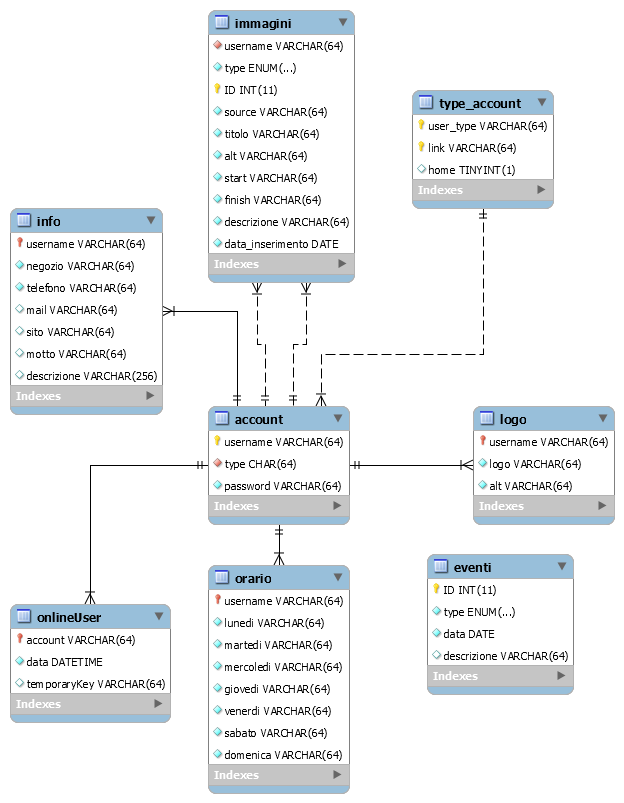
\includegraphics[width=0.8\linewidth]{images/diagram}\\
\end{center}
\vskip1cm
\newpage

\subsection{Validazione dei Form}
La parte di amministrazione e inserimento contenuti del sito è ricca di form, quindi si avranno avvisi sia in javascript sia in html riguardanti gli errori trovati nei campi di inserimento durante la procedura di invio dei dati; gli avvisi in php avverranno rispetto alla parte javascript nella parte alta della pagina, indicando la tipologia di errore rilevata o l'avvenuto inserimento dei dati in modo corretto.\\
Le funzioni di validazione dei form sono create ad hoc, poichè essendo esse molto poco omogenee come richieste non danno la possibilità di raggruppare in un'unica funzione tutti i controlli da svolgere.\\
L'assenza di javascript non è problematica per il controllo di tali form, poichè gli appositi controlli vengono svolti quantomeno da una funzione server-side in php prima di salvare i dati nel database.\\
\subsection{Dimensionamento immagini}
Le immagini inserite vengono scalate appositamente affinchè non vi siano problemi nella loro visualizzazione all'interno del sito. Tale funzionalità è stata inserita per evitare di dover vincolare ad una dimensione fissata l'inserimento delle immagini nel sito. Nell'eventualità in cui le immagini non venissero scalate nel modo desiderato è sempre possibile sostituirle con un'altra immagine correttamente dimensionata prima dell'inserimento nel sito.

\section{Compatibilità}
Durante lo sviluppo del sito è stato chiaro sin dal primo momento che fosse necessario supportare un'ampia gamma di browser per accedere al sito.
\\I browser che sono stati testati e controllati per il corretto funzionamento del sito sono:
\begin{itemize}
	\item Chrome - Versione 67.0.3396.99 
	\item Mozilla Firefox - Versione 61.0
	\item Opera - Versione 54.0.2952.41
	\item Microsoft Edge - Versione 42.17134.1.0
	\item Internet Explorer 11- Versione 11.112.17134.0
	\item Internet Explorer 9 (emulato tramite Microsoft Edge)
\end{itemize}

\section{Test e validazione}
\subsection{Introduzione}
Questa sezione è dedicata alla sintesi dei test effettuati e alla descrizione degli strumenti utilizzati a tale scopo.\\
Preso atto che gli strumenti automatici non sono in senso assoluto un indicatore sufficiente per definire un sito accessibile, essi sono un requisito necessario per poter affermare che il nostro sito sia quantomeno conforme alle linee guida consigliate.\\
Poichè il sito permette il caricamento di contenuti il risultato di alcuni test, con particolare riferimento ai colori, potrebbe non essere lo stesso se eseguito una volta popolato il sito. L'esito di questi test è quindi valido soltanto nelle parti esenti dal caricamento di immagini degli utenti.
\subsection{Validazione}
\subsubsection{Strumenti utilizzati}
\begin{itemize}
	\item \textbf{W3C Validator}: servizio di validazione del markup disponibile al link:\\
	\url{https://validator.w3.org/};
	
	\item \textbf{Total Validator}:validatore di accessibilità e correttezza del markup disponibile in versione gratuita al sito:\\
	\url{http://www.totalvalidator.com/validator/Validator};
	
	\item \textbf{NVDA}: screen reader reperibile gratuitamente al link:\\
	\url{https://www.nvaccess.org/};
	
	\item \textbf{IE Accessibility Toolbar}: barra di strumenti per test di accessibilità compatibile solo con internet Explorer ed installabile al sito:\\
	\url{https://developer.paciellogroup.com/resources/wat/};
	
	\item \textbf{Let's get color blind}: plugin per browser utile per simulare il daltonismo; permette di visualizzare come il sito viene visto da un individuo affetto da Protanopia, Deutanopia, Tritanopia e Achromatopsia, disponibile gratuitamente al sito:\\
	\url{https://addons.mozilla.org/en-US/firefox/addon/let-s-get-color-blind/};
	
	\item \textbf{WebAIM Color Contrast Checker}: validatore di contrasto del colore disponibile gratuitamente al sito:\\
	\url{https://webaim.org/resources/contrastchecker/};
\end{itemize}
\subsubsection{Esiti}
\begin{itemize}
	\item \textbf{W3C Validator}: Tutte le pagine sono state validate e non risulta che esse abbiano errori di validazione del codice.
	
	\item \textbf{Total Validator}: le reportistiche del validatore hanno portato al miglioramento e all'adeguamento di alcuni elementi che non rispondevano  ai criteri delle linee guida WCAG 2.0 AAA.\\
	Il sito allo stato attuale non porta con se errori di validazione, garantendo almeno sulla carta il massimo livello di accessibilità possibile.
	
	\item \textbf{NVDA}: pur con la consapevolezza che la prova non sia esauriente, il sito è stato testato con lo screen reader NVDA e gli aiuti alla navigazione inseriti sono risultati
	propriamente funzionanti.
	
	\item \textbf{IE Accessibility Toolbar}: il sito è stato testato utilizzando le seguenti funzionalità integrate all'interno di questo strumento:
	\begin{itemize}
		\item Color Contrast Analyser: è stato verificato che i colori del sito sono conformi ai livelli di accessibilità definiti da WCAG 2.0 AAA.
		
		\item Juicy Studio Analyser: questo strumento effettua un' analisi riguardo all'accessibilità basandosi sul livello di contrasto dei colori che individua.\\
		Il sito non presenta problematiche di questo tipo, in particolar modo con un livello di contrasto mai sotto il valore di 7:1 vengono appieno soddisfatte le direttive per il livello AAA di accessibilità dal punto di vista del contrasto del colore.\\
		Unica problematica rilevata da questo strumento è il livello di contrasto del link per accesso rapido al contenuto della pagina, volutamente reso trasparente all'utente e visibile solo durante l'utilizzo di strumenti come gli screen reader.
	\end{itemize}
		
	\item \textbf{WebAIM Color Contrast Checker}: dati due colori, uno relativo al contenuto in
	primo piano e uno relativo al conteuto in secono piano, il validatore restituisce un
	indice di contrasto con il quale verifica l’accessibilità della combinazione di colori
	secondo WCAG AA e WCAG AAA. I colori del sito sono stati scelti in modo tale
	da essere conformi a WCAG AAA.
	
\newpage	
	\item \textbf{Toptal Colorblind Web Page Filter}: la simulazione del daltonismo dato da protanopia (non percezione del rosso) è forse la più ostica poichè il sito si basa sul colore rosso; fortunatamente non vi sono difficoltà di contrasto soprattutto nei menù, con un contrasto sempre sufficiente per il riconoscimento degli elementi.\\
	\vskip1cm
	\begin{center}
		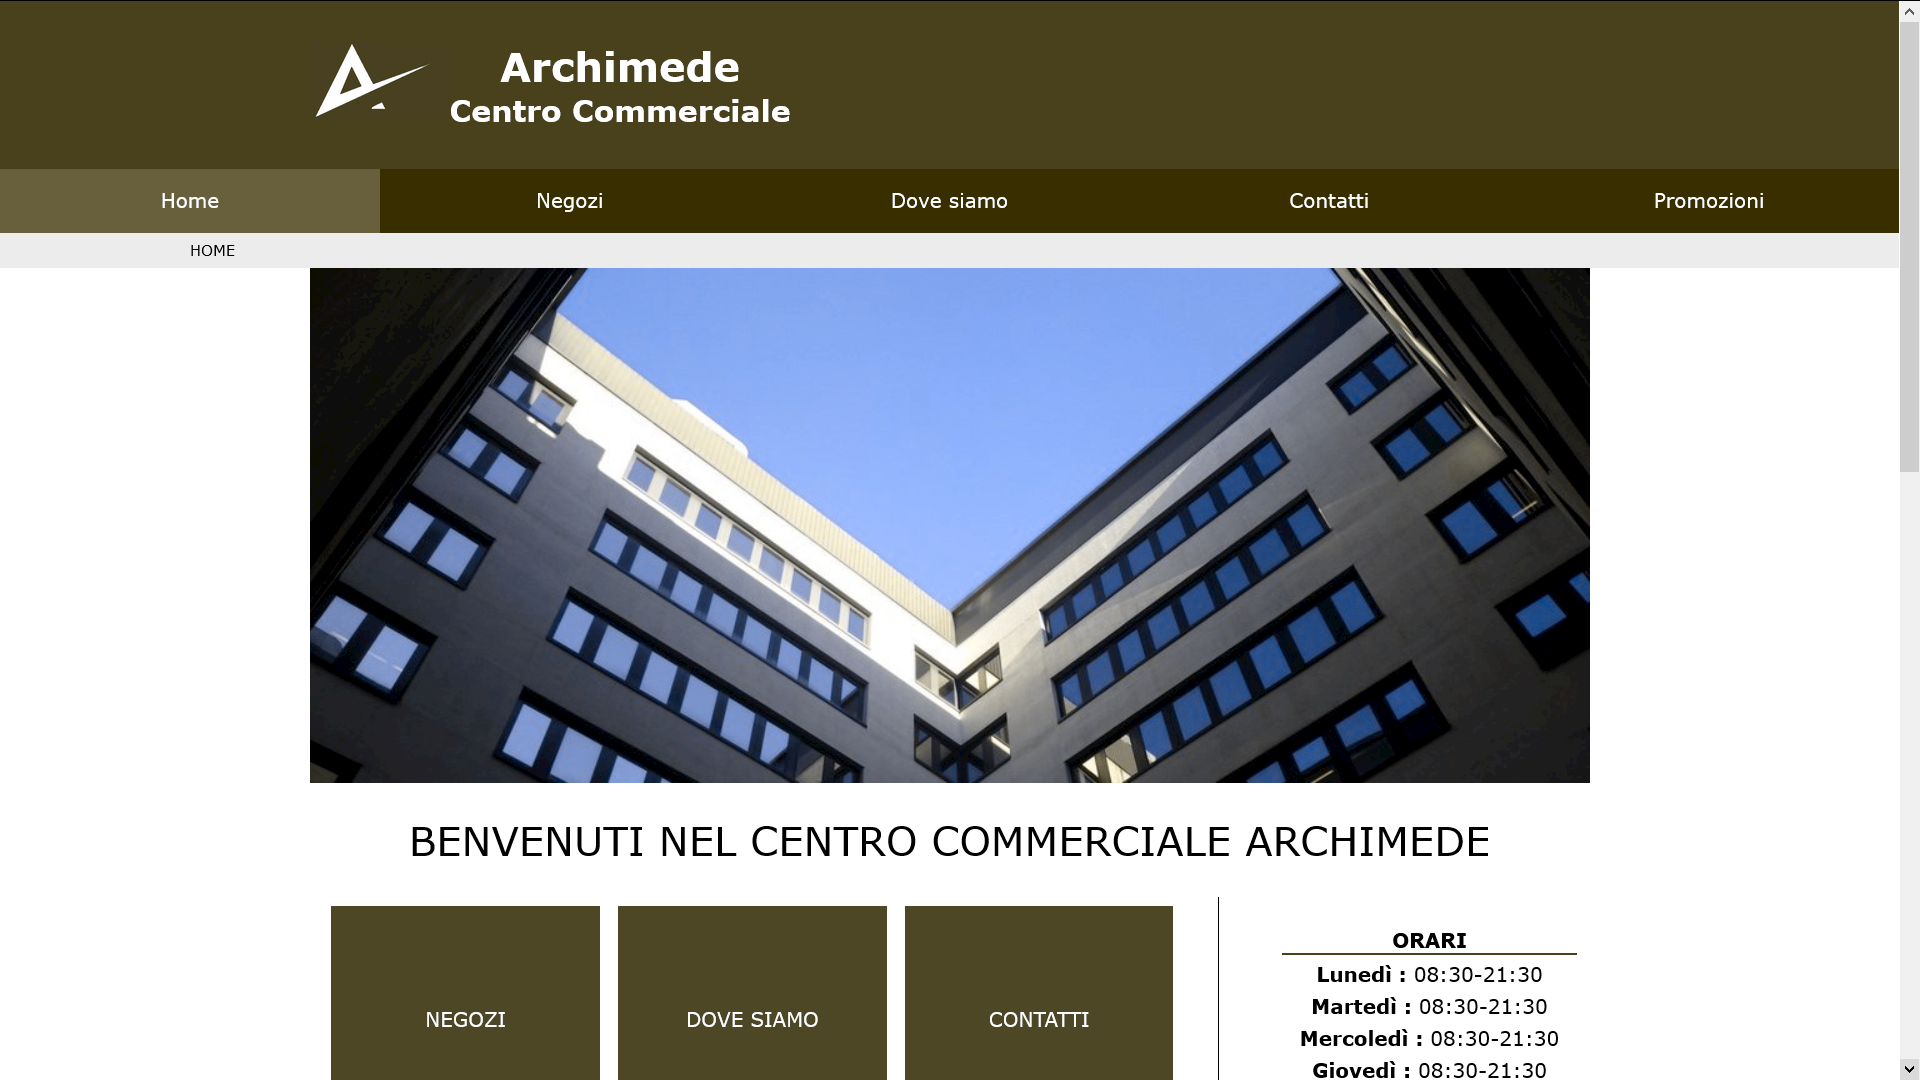
\includegraphics[width=0.7\linewidth]{images/protanopia}\\
		\vskip1cm
		- Home del sito per persone affette da protanopia
	\end{center}
	\vskip1cm
	Il daltonismo da deuteranopia (non percezione del verde), tritanopia (non percezione del blu) e achromatopsia (non percezione del grigio) non dà complicazioni particolari, anche perchè tali colori non sono presenti sul sito in modo visibile.
	\vskip1cm
	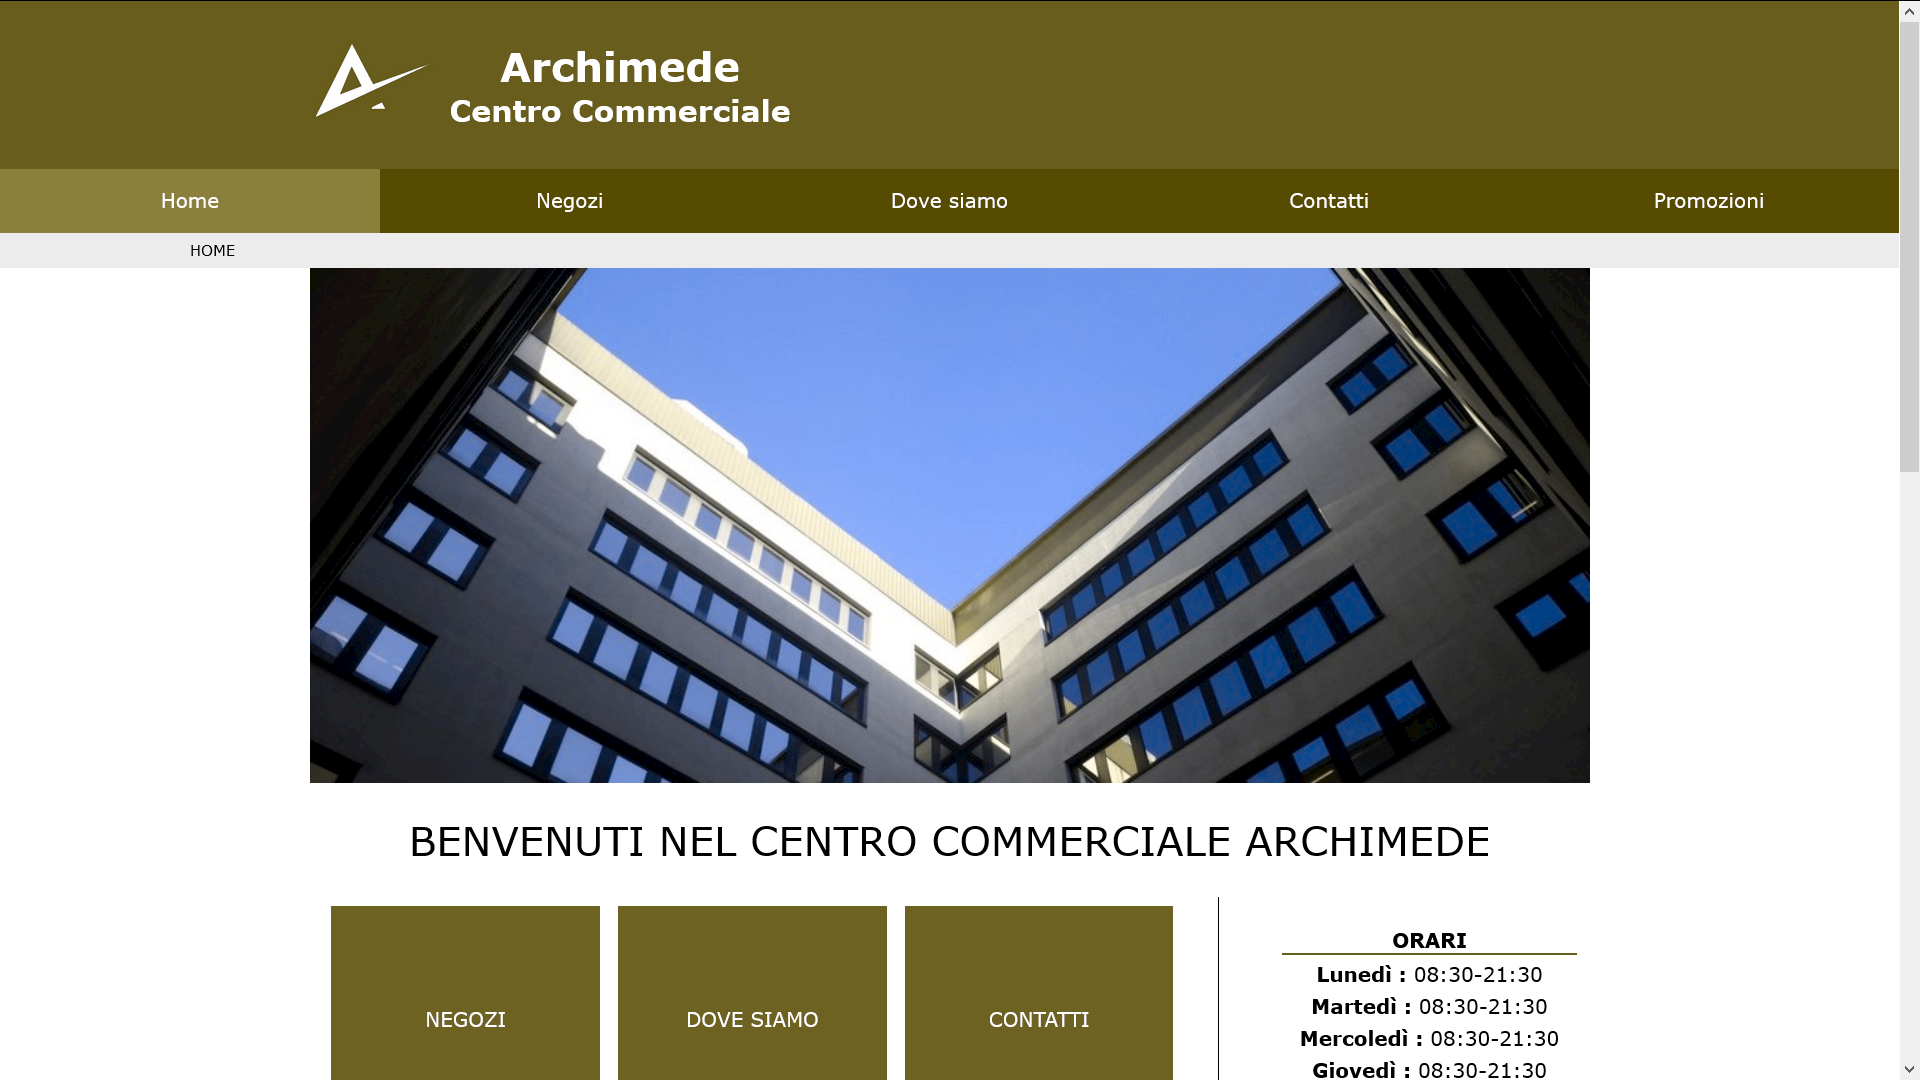
\includegraphics[width=0.3\linewidth]{images/deuteranopia}
	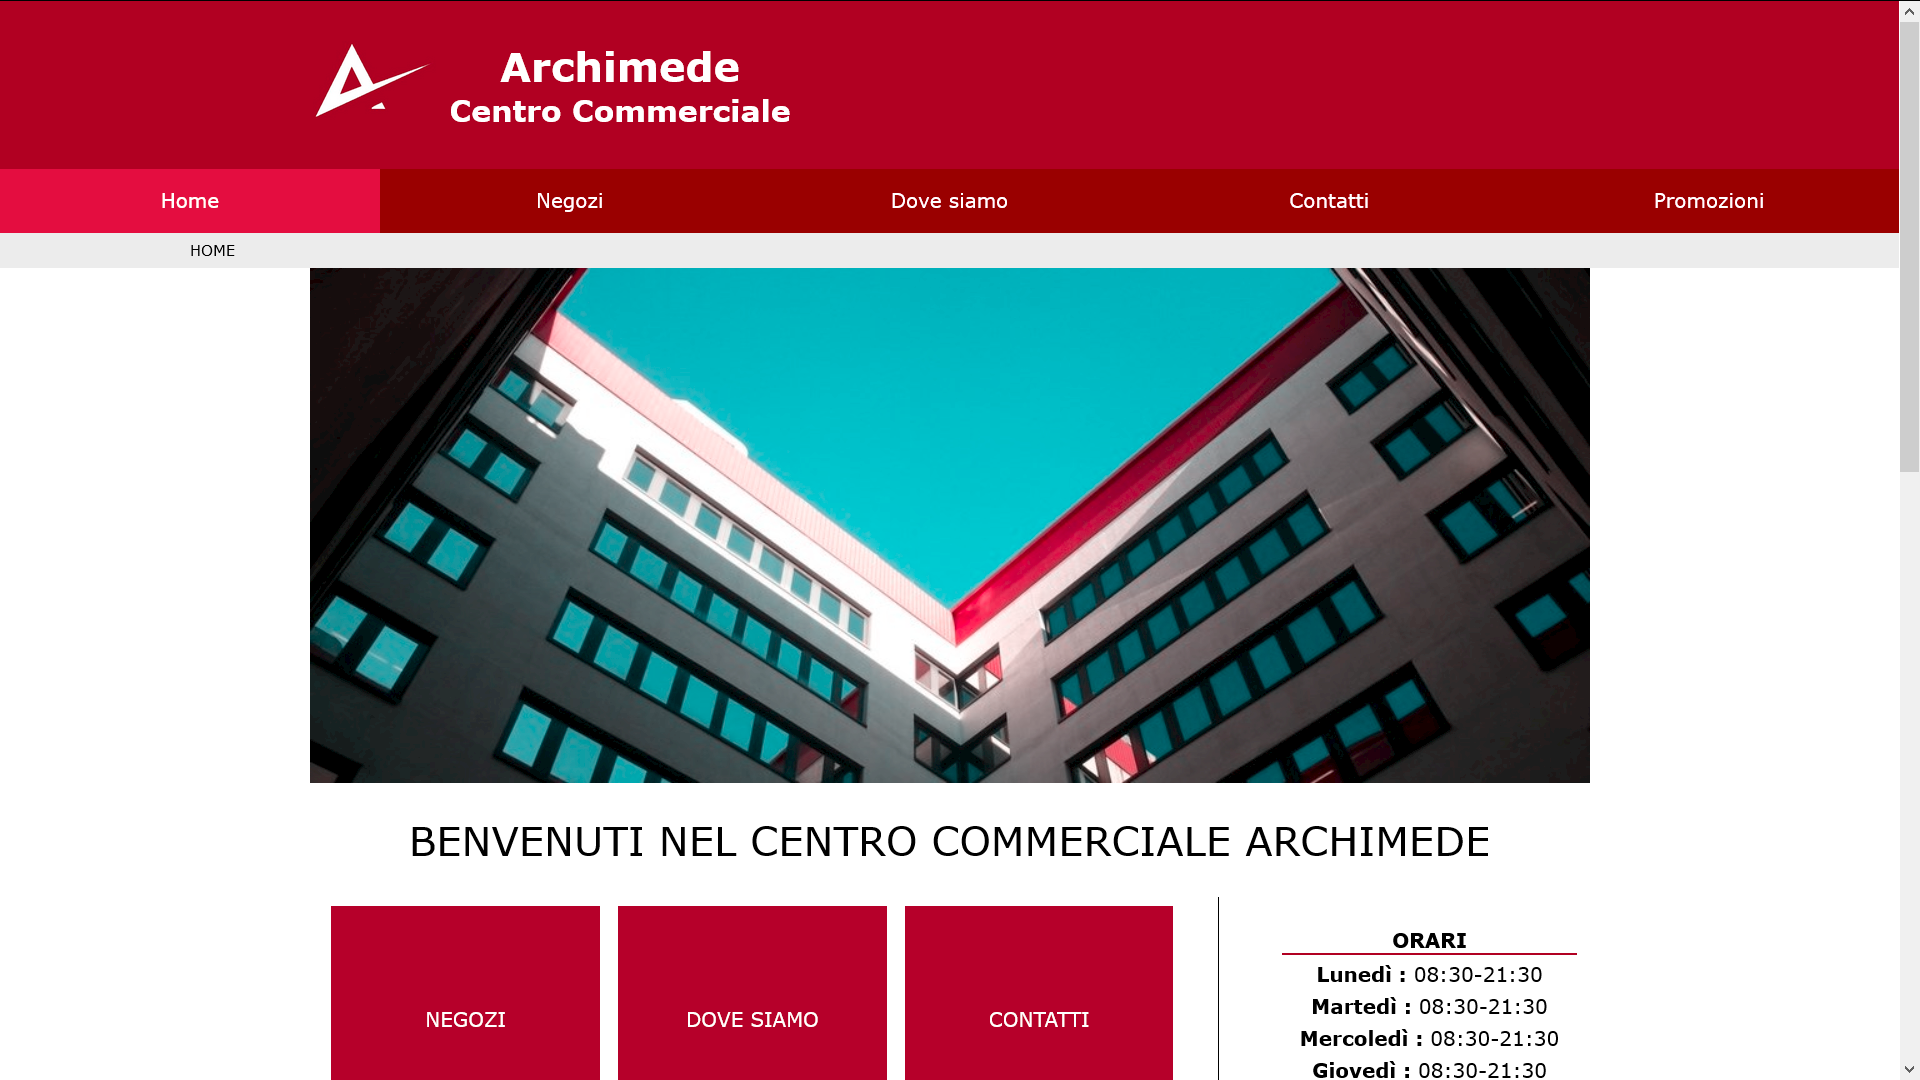
\includegraphics[width=0.3\linewidth]{images/tritanopia}
	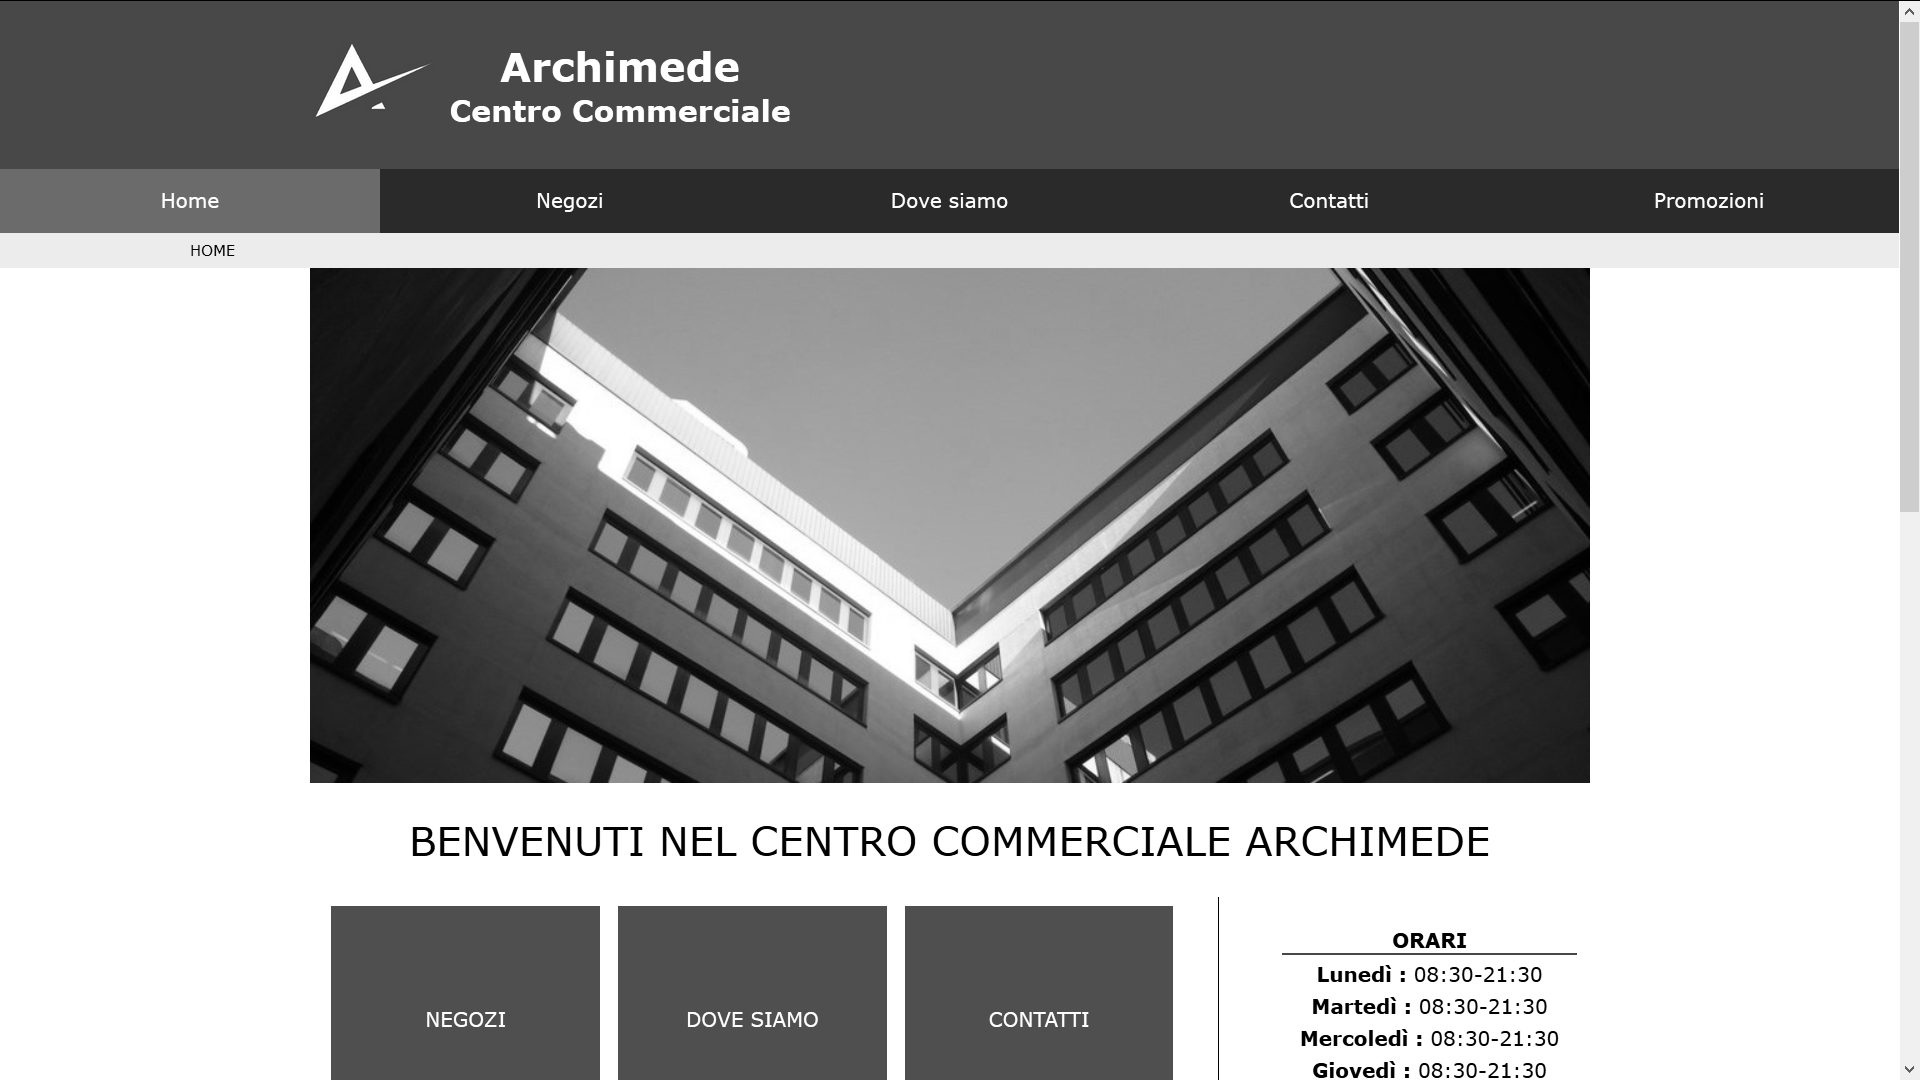
\includegraphics[width=0.3\linewidth]{images/achromatopsia}\\
	\vskip1cm
	- Home del sito per persone affette rispettivamente da deuteranopia, tritanopia e achromatopsia.
	
	\end{itemize}
\newpage
\subsection{Performance}
\subsubsection{Strumenti}
 \begin{itemize}
 	\item \textbf{Performance test Opera Browser}: strumento integrato nel browser Opera per la verifica in background della velocità di caricamento e rendering delle pagine web;
 	\item \textbf{Google PageSpeed Insights}: suite di test per la verifica della velocita di caricamento del sito da dispositivi mobile e desktop, disponibile al sito:\\
 	\url{https://developers.google.com/speed/pagespeed/insights/?hl=it};
 	\item \textbf{GTmetrix}: analizzatore di performance per siti web, disponibile al sito:\\
 	\url{https://gtmetrix.com/}.
 \end{itemize}
\subsubsection{Esiti}
\begin{itemize}
	\item \textbf{Performance test Opera Browser}: il performance test ha dato come esito una velocità di caricamento di 9.9 ms nel caricamento della pagina home e una velocità di rendering di 13.6 ms per un totale di 23.5 ms per il caricamento completo della pagina web, un tempo tale da non consentire neanche di vedere l'animazione di caricamento della pagina (che si attiva soltanto in presenza di particolari connessioni molto lente).
	\item \textbf{Google PageSpeed Insights}: il test ha avuto esito positivo riportando come risultato una "buona" velocità per dispositivi desktop e mobile.
	\item \textbf{GTmetrix}: il test ha avuto un buon esito, risultando nella velocità delle pagine di livello "A"
\end{itemize}
\newpage
\subsection{Usabilità}
\subsubsection{Strumenti}
\begin{itemize}
	\item \textbf{Google Mobile Friendliness Test}:suite di test per la verifica dell’usabilità del	sito da dispositivi mobile, disponibile al sito:\\
	\url{//https://search.google.com/test/mobile-friendly};
	\item \textbf{Test umano}: test condotto da alcuni candidati senza particolari conoscenze informatiche a cui è stato richiesto di reperire determinati contenuti all’interno del sito
\end{itemize}
\subsubsection{Esiti}
\begin{itemize}
	\item \textbf{Google Mobile Friendliness Test}: l'esito di tale test è stato positivo, poichè tale strumento ha valutato il sito "mobile friendly". L'esito del test può comunque variare leggermente nei risultati di punteggio in base al numero di tentativi ravvicinati che possono essere richiesti per la verifica del sito.
	\item \textbf{Test umano}: sia da piattaforma mobile che da piattaforma desktop è stato selezionato un campione di 5 persone di diverse età con conoscenze informatiche per quanto possibile basilari. Il test, consistente nella ricerca di vari contenuti all'interno del sito, si è concluso in modo positivo poichè nessuna persona si è persa all'interno del sito e ha raggiunto rapidamente i contenuti ricercati.
\end{itemize}
\newpage
\section{Suddivisione dei lavori}
Tenendo conto del fatto che ogni elemento del gruppo ha contribuito allo sviluppo e alla verifica del materiale prodotto dai propri colleghi, i lavori sono stati distribuiti nel modo seguente:
\begin{itemize}
	\item Giovanni Bergo: sviluppo dell'interfaccia della parte privata, con particolare riferimento agli script Javascript per i controlli delle form e all'interfaccia della parte admin; realizzazione del css per la stampa (print.css).
	\item Bianca Ciuche: sviluppo dell'interfaccia della parte pubblica, realizzazione dello stile per l'utilizzo di dispositivi mobile e tablet, validazione delle pagine e adattamento del sito ai criteri di accessibilità.
	\item Manfredi Smaniotto: sviluppo dell'interfaccia della parte privata con particolare riferimento alla parte negozi, scrittura della relazione e realizzazione dei test di accessibilità del sito.
	\item Daniel Rossi: realizzazione del database e gestione delle transazioni con esso nella parte di back-end, realizzazione dei controlli e degli adattamenti dei contenuti delle form in PHP e realizzazione del caricamento dinamico del sito.
\end{itemize}

\end{document}